%
%
%   S A I J O  2
%
%

% created by kadono 2018/11/25 01:00
% edited by nakayama 2018/11/25 2:00

\documentclass[11pt,b5paper,papersize,dvipdfmx]{jsbook}

\usepackage{vuccaken}
\usepackage{vuccaken2018}
\usepackage{15saijo}


% 以下本文
\begin{document}

% - - - - - - - - - - - - - - - - - - - - - - -
\kaishititle{ゼロから始める飛行の書}%
                {機械工学科1回生}{西條晴幸}
% - - - - - - - - - - - - - - - - - - - - - - -
% 遠くまで飛ぶ紙飛行機の翼の形とは \\
% -揚抗比測定装置の作成-

%
\section*{はじめに}
最近話題になっている小型無人機「ドローン」について、飛行機型のドローンの開発について考えた。大き目な紙飛行機サイズのオーダーだ。飛行機型のドローンの難点は、ヘリコプター型のものと比べ安定性が低く、機体形状や制御の開発にコストがかかることである。よって、翼の形状の評価を行うことができる装置を、安価に作成することを試みた。またこのサイズ感と実験の簡単さと私の趣味で、まずは紙飛行機の翼型について調べられるような装置を作ることとした。作成した装置を用いて、2種類の翼型について評価を行ったところ、相対的に、理論結果に近い結果が得られた。このことより、紙飛行機が飛ぶと考えられる流れ場において、目安となる翼の評価を行える装置を作成できたと言える。装置の作り方について丁寧に記述したので、自由研究くらいにでも使っていただければと思う。

\section{目的}
二次元翼の陽抗比を求められる簡易で低コストな実験装置を作成し、その装置の有用性を調べる。
\section{揚抗比測定装置の作成}
風路など主な部分の作成方法は,
JAXA宇宙教育センター,―ミニ風洞― \url{http://edu.jaxa.jp/materialDB/detail/78875}
を参考にし、若干の改変を加えた。つまり、簡便な風洞実験装置の作成を試みる。
\subsection{準備物}

\renewcommand{\labelenumi}{[\arabic{enumi}]}
\begin{enumerate}
  \item 空冷ファン:1 辺が12\ cm、厚さ40\ mm 程度。\\
  厚さ20\ mm程度の出力がやや小さいものしか入手できない場合は、それでもよい。その際は[10]のボルトの長さは首下長さ30\ mmでよい。電子部品のパーツセンターなどで購入できます。パソコン用のファンではパワーが不足するため、電子装置用の冷却ファンを用いることが望ましい。AC100V駆動のものを用いる場合は別途電源コードを用意する必要がある。\\
  今回使用したファンは長尾製作所「X-FAN RDH1238B」である。電源はPCの電源装置より4ピン接続で用いた。
  \item 120\ mmFAN用フィンガーガード(上記[1]空冷ファンの防護フェンス)
  \item バルサ板またはベニヤ板\\
  風路用:120$\times$360$\times$厚さ13\ mm を2枚、146$\times$360$\times$厚さ13\ mmを2枚
  \item の空冷ファンをちょうど入れることができる長さ360mm の四角い筒が作れれば、寸法は自由でよい。\\
  翼の模型用:146$\times$100$\times$厚さ13\ mm 任意枚
  \item 厚めの工作用紙あるいはプラスチックの下敷:40$\times$120\ mmの長方形10枚
  \item 竹串:長さ136\ mm、直径3\ mm任意本(制作する翼の枚数の2倍数)
  \item 画用紙:48$\times$100\ mm数枚
  \item 木ねじ:3.2$\times$32\ mm、16本
  \item ベニヤ板:厚さ3\ mm 程度、1辺が60\ mmの直角2等辺三角形4枚
  \item ボルト:M4 首下長さ50\ mmのもの、ナット、スプリングワッシャ4組
  \item 木ねじ:3$\times$12\ mm 12本
\end{enumerate}
  [工具など]\\
  木工用きり若しくはドリル,ドライバー,はさみ,速乾性木工用接着剤,カッター
  \newpage
\subsection{作成手順}
\subsubsection{作成手順}
\begin{enumerate}
\renewcommand{\labelenumi}{\Roman{enumi}).}
\item $[3]$の板($120\times 360\times 13$\ mm\ 2 枚、$146\times 360\times 13$\ mm\ 2 枚)を使って、[1]の空冷ファンをぴったり入れることができる長さ360\ mm の四角い風路を作る。(下図\ref{fig:zuiti}参照)
\begin{figure}[H]
  \centering
  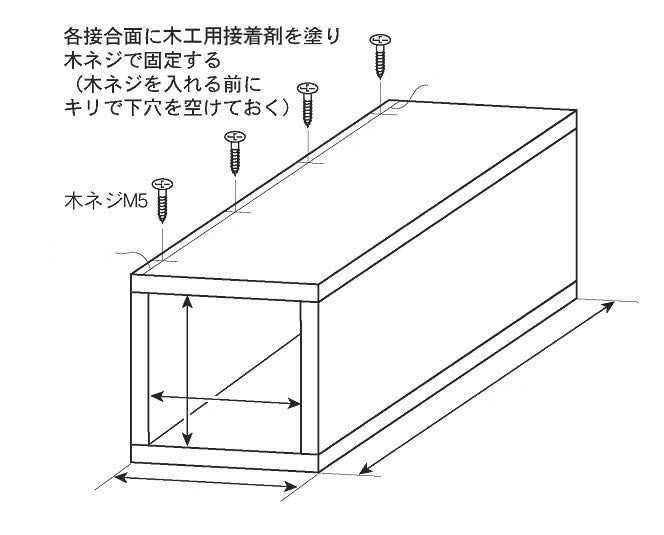
\includegraphics[width=7cm]{saijo2/img/zuiti.PNG}
  \caption{}
  \label{fig:zuiti}
\end{figure}
\item 板の組み合わせを確認した後、木工用きり若しくはドリルで木ねじ用の下穴を100~mm 間隔であける(下穴をあけておかないと板が割れることがある)。板の接合面を木工用接着剤で貼り合わせ、乾燥する前に[8]の木ねじで固定する。
\item 空冷ファンを風路のいちばんはしに挿入する。
\item 空冷ファンを固定する。
  \begin{enumerate}
    \renewcommand{\labelenumii}{\alph{enumii}).}
    \item 空冷ファンの4か所の角部に固定用の穴があるため、その穴に合わせて[9]の三角形のベニヤ板にボルトを通す穴をあける。その際、ベニヤ板の直角の角が、風路の外側の角部に合うように穴の位置を決める(下図\ref{fig:zuini}参照)。
    \item 固定は風路の外側から[2]の防護フェンス、三角板、空冷ファンの順にボルトを通し、風路内側に出たボルトのはしには、スプリングワッシャ、ナットを通し、外側からドライバーで締める。(下図\ref{fig:zuini}参照)。
    \begin{figure}[H]
      \centering
      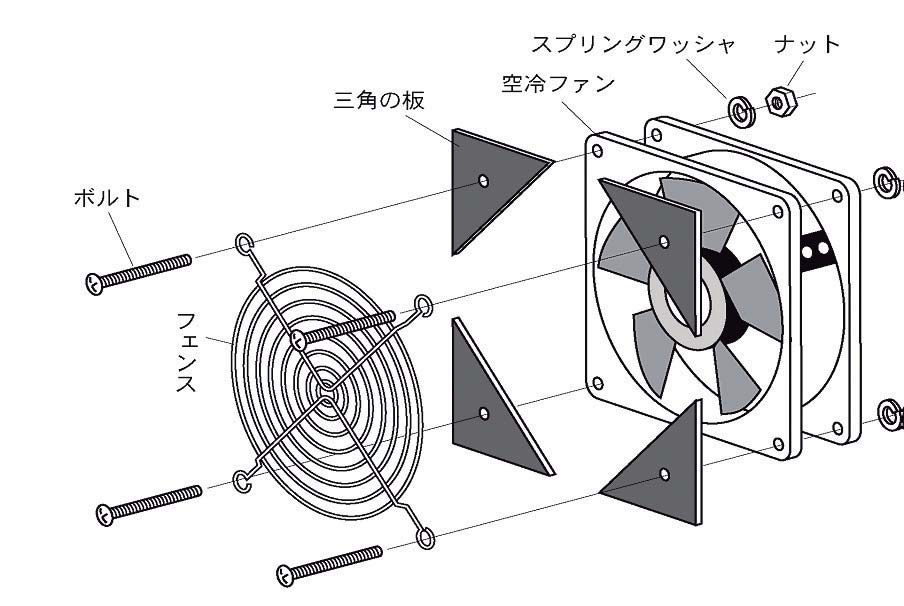
\includegraphics[width=7cm]{saijo2/img/zuni.PNG}
      \caption{}
      \label{fig:zuini}
    \end{figure}
    \item 空冷ファンとベニヤ板の位置が決まったら、[11]の木ねじでベニヤ板をそれぞれ
    3か所で固定する。(下図\ref{fig:zusan}参照)
    電線が外に取り回せないファンの場合、風路に電線を出す穴を設ける。
    \begin{figure}[H]
      \centering
      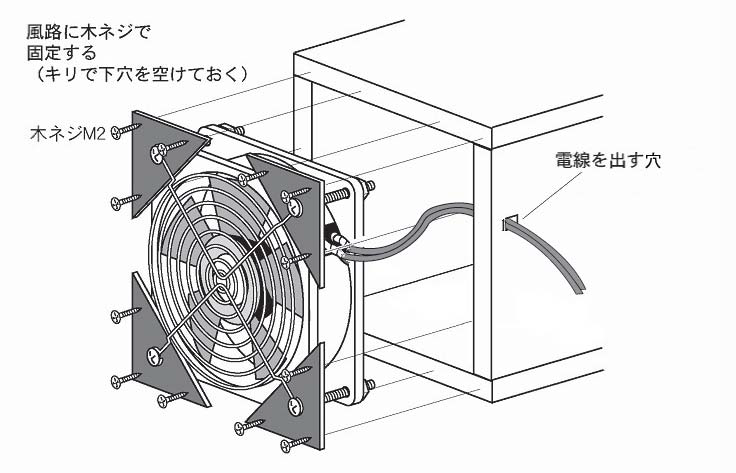
\includegraphics[width=7cm]{saijo2/img/zusan.PNG}
      \caption{}
      \label{fig:zusan}
    \end{figure}  
  \end{enumerate}
\item $[4]$の工作用紙あるいはプラスチックの下敷を使って整流格子を作る。
  \begin{enumerate}
    % \renewcommand{\labelenumii}{\alph{enumii}).}
    \item 短辺のはしから20\ mm間隔で、長辺に垂直に20\ mm、直線を5本引く。次に右側から、はさみなどで線にそって切り込みを入れる。
    \item 縦横に組み合わせて、格子の穴の寸法が一辺20\ mm奥行き40\ mm の格子を作り、組み合わせた部分を木工用接着剤で適当に固定する。
    \begin{figure}[H]
      \centering
      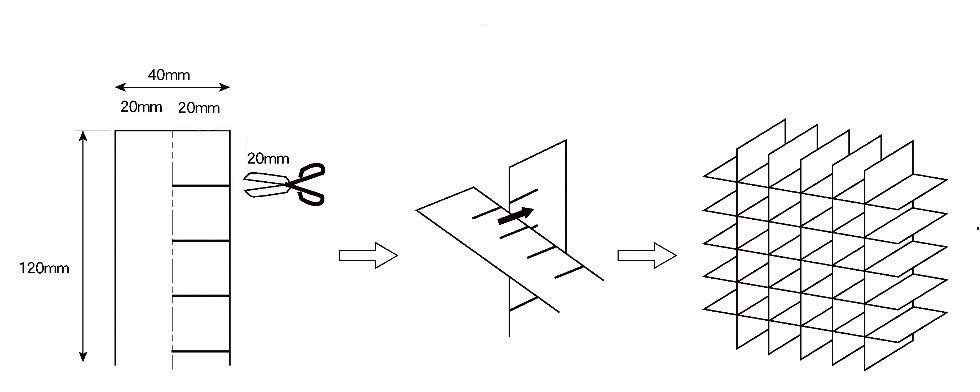
\includegraphics[width=7cm]{saijo2/img/ziyon.PNG}
      \caption{}
      \label{fig:zuyon}
    \end{figure}
    \item 接着剤が乾いたら、風路の中、空冷ファンの側と反対側のはしから240~mm 以上奥の位置に差し入れる(下図\ref{fig:zugo}参照)。あとで取り替えができるように軽く接着しておく。  
    \begin{figure}[H]
      \centering
      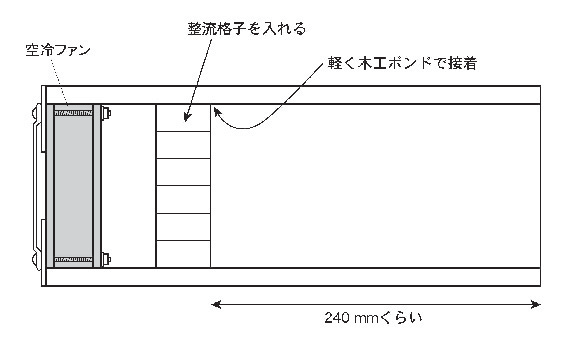
\includegraphics[width=7cm]{saijo2/img/zugo.PNG}
      \caption{}
      \label{fig:zugo}
    \end{figure}
  \end{enumerate}

\end{enumerate}




\section{実験}
\subsection{実験手法}
翼作成の簡易性を鑑み、実験を行う翼は翼型が直線の直線型と、翼型が中折れ型とした。また各翼型を飛行物体に使用した際に公平に扱うため、重量(この場合翼の前端から後端までの翼にそった弓なりの長さ)を揃えた。
また空気の流れに対する迎え角は$10^\circ$とする。\par
この条件下で、それぞれの翼について装置を用いて揚力と抗力をそれぞれ5回測定し、最大値と最小値を除いた3回の平均値を結果の値とする。
\subsection{実験環境}
本実験は室内で行う。
実験時の気圧は1013\ hPa。
また今回使用したファンで生み出される風速を計算しておく。
今回使用した,長尾製作所「X-FAN RDH1238B」の風量は$154.0\ \mathrm{CFM}$(立法フィート毎秒)である。また、風路は$12\ \mathrm{cm}$四方である。また、$1\ \mathrm{ft^3}= 28 316.846 592 \mathrm{cm^3}$より求められる風速(m/s)は,
\begin{align*}
  154 \times \frac{28316.846592}{12^2\times 100\times 60} = 5.047215712\ \rm{(m/s)}
\end{align*}
約5\ m/sとなる。紙飛行機の滑空速度はおよそ$4\sim 5$\ m/sであるため、この風速は紙飛行機の実験を行うにあたって適切なものだと言える。\par
 また本実験環境において、空気の流れは乱流である。ここにレイノルズ数を示す。\par
(レイノルズ数:流体の慣性力と粘性力の比を表す無次元数であり、流れ場の性質を示す指標として用いられる。)


\begin{itemize}
  \item[] \hspace{-2zw}{\bf [文字の定義と値]}
  \item $U$(代表流速):本実験では風速にあたるため,事前計算よりおよそ5\ m/sである。
  \item $L$(代表長さ):本実験では翼弦長にあたるためおよそ0.06\ mである。
  \item $\rho$(流体の密度):本実験では室内の空気の密度。気圧$P = 1013\ \rm{hPa}$、室温$t =27^\circ \rm{C}$、乾燥空気の気体定数$R (= 2.87)$、機体の状態方程式$P=\rho R(t+273.15)$よりこれを$\rho$について解くと$\rho = P/\{R(t+273.15)\}$なので数値を代入して$\rho=1.175950932778935$である。
  \item $\mu$(流体の粘性係数):本実験では空気の粘性係数にあたり、$27^\circ \rm{C}$において引用[8]より$1.830\times 10^{-5}$である。
\end{itemize}

まとめるとそれぞれ
\begin{align*}
  U \fallingdotseq 5.0\ \rm{m/s},&\quad
  L \fallingdotseq 0.060\ \rm{m},\\
  \rho \fallingdotseq 1.176\times 10^3\ \rm{kg/m^3},&\quad
  \mu \fallingdotseq 1.83\times 10^{-5}
\end{align*}
よってレイノルズ数$Re$は
\begin{align*}
  Re = \frac{\rho vL}{\mu} &= \frac{5.05 \times 0.0600 \times 1.176 \times 10^3}{1.830\times 10^{-5}}\\
  &= 19471475.40983607 \fallingdotseq 1.95 \times 10^7
\end{align*}
この値から、本実験環境における流れ場は層流ではなく乱流であることがわかる。このため残念ながら理論計算することは難しく、各数値単体での正当性の検証は困難である。

%
\section{結果}
\begin{minipage}{0.45\hsize}
  \begin{center}
    {\bf 直線型}\\
    揚力$\cdot \cdot \cdot$2.7g\\
    抗力$\cdot \cdot \cdot$0.6g\\
    揚抗比$\cdot \cdot \cdot$約4.50\\
  \end{center}
\end{minipage}
\begin{minipage}{0.45\hsize}
  \begin{center}
    {\bf 中折れ型}\\
    揚力$\cdot \cdot \cdot$6.1g\\
    抗力$\cdot \cdot \cdot$0.9g\\
    揚抗比$\cdot \cdot \cdot$約6.78
  \end{center}
\end{minipage}

%
\section{考察}
5回のいずれの試行においても数値の誤差は$\pm 0.6$\,g程度であったため、精度の高い実験ができたと考えられる。\par
二つの翼の揚抗比は多くの航空機に用いられているように、低速域において中折れ型のほうが大きい値を示すことがわかっている。実験結果の数値はこの事実に沿っており、このことからこの装置は目安程度には信頼できる揚抗比を測定できるものだと考えられる。\par
また今回の実験の全予算は測定装置(キッチンスケール2500円)も含め7000円程度であり、十分な低コスト化に成功したと言える。
 
%
\section{結論}
二次元翼の陽抗比を求められる実験装置を低コストで作成し、その正確性の程度を実験によって示すことができた。

%
\section{今後の課題}
装置の有用性の証明にはまだ数パターンの翼についての評価を行うことも必要であるため、より信頼性の高い結論を示すために実験を繰り返すことを今後の課題とし、そこから速度域を上げてドローン開発に向けていく。

\clearpage

% 参考文献
\sanko
\begin{enumerate}
  \item 小林 昭夫「紙ヒコーキで知る飛行の原理―身近に学ぶ航空力学」(1988)
  \item 須藤 浩三「流体の力学」コロナ社
  \item JAXA宇宙教育センター,―ミニ風洞―\\
    \url{http://edu.jaxa.jp/materialDB/detail/78875}
  \item 飛行機はなぜ飛べるか? 揚力とは? キャンバの効果のメカニズムとは?\\
    \url{http://www2.plala.or.jp/puthoff/wing.html}
  \item 飛行機に働く力basic forces;lift, drag, thrust 航空実用辞典\\
    \url{http://www.jal.com/ja/jiten/dict/p051.html}
  \item 水理学  株式会社環境技術研究所開発センター\\
    \url{http://spokon.net/eelnews/hydraulics/009s.htm}
  \item 流体解析の基礎講座 ソフトウェアクレイドル\\
    \url{http://www.cradle.co.jp/tec/column01/008.html}
  \item 標準大気の特性 HEISHIN\\
    \url{http://www.eng-book.com/sample/pdf/eb18_p150.pdf}
  \item 流体力学 水・空気の物性 機械用語集 \\
    \url{http://www.mterm-pro.com/machine-yougo/}\\
    \qquad\qquad\url{fluid-dynamics/water-air-bussei.html}
  \item 流体解析の基礎講座 第$1\sim8$回\\
    \url{http://www.cradle.co.jp/tec/column01/}
  \item パッと知りたい! 人と差がつく乱流と乱流モデル講座 第$1\sim13$回\\
    \url{http://www.cradle.co.jp/tec/column04/index.html}
\end{enumerate}


\end{document}
%
% ファイトだよ!
%